\documentclass{article}

\usepackage{amsmath}
\usepackage{amsthm}
\usepackage{graphicx}


\newtheorem{algorithm}{Algorithm}
\setlength\parindent{0pt}

\title{Group Assignment 3}
\author{Chance Zibolski, Dean Johnson}

\begin{document}
\maketitle

\section{Pseudocode for 3 methods}
\begin{verbatim}
Method1(a[0,...,n-1], b[0,...,m-1])
    best_a = n-1
    best_b = 0
    for i = 0; i < n; i++
        for j = 0; j < m; j++
            best = abs(a[best_a] + b[best_b])
            curr = abs(a[i] + b[j])
            if curr < curr_best
                best_a = i
                best_b = j
    return (best_a, best_b)
\end{verbatim}

\begin{verbatim}
Method2(a[0,...,n-1], b[0,...,m-1])
    best_a = n-1
    best_b = 0
    a = sort(a)
    b = sort(b)
    for i = 0; i < n; i++
        last = infinity
        for j = 0; j < m; j++
            curr = abs(a[i] + b[j])
            if curr > last
                break
            last = curr
            best = abs(a[best_a] + b[best_b])
            if  curr < best
                best_a = i
                best_b = j
    return (best_a, best_b)
\end{verbatim}

\begin{verbatim}
Method3(a[0,...,n-1], b[0,...,m-1])
    new_list = a
    append negation of list b to new_list
    new_list = sort(new_list)

    best_a = -1
    best_b = -1
    for i = 0; i < n+m-2; i++
        curr, next = new_list[i], new_list[i+1]

        if curr and next are both in same original list
            continue

        diff = abs(curr - next)

        if (best_a != -1 and best_b != -1) and diff < abs(best_a - best_b)
            best_a = curr
            best_b = next

    return original indices of best_a and best_b
\end{verbatim}

\section{Pseudocode for a divide and conquer algorithm for closest to zero problem}
\begin{verbatim}
sum_of_suffices(a[0,...,n-1])
    for i = n-2; i > 0; i--
        a[i] = a[i] + a[i+1]
    return a

sum_of_prefices(a[0,...,n-1])
    for i = 1; i < n; i++
        a[i] = a[i] + a[i-1]
    return a

ctz(a[0,...,n-1], suffix_prefix_method)
    if n < 2
        return a[0]

    left = a[0,..,n/2]
    right = a[(n/2)+1,..,n-1]

    sum_left = ctz(left)
    sum_right = ctz(right)

    suffices = sum_of_suffices(left)
    prefices = sum_of_prefices(right)

    // suffix_prefix_method is the subroutine chosen
    sum_both = suffix_prefix_method(suffices, prefices)

    val = min{
        sum_left,
        sum_right,
        sum_both
    }

    return val, indices (i, j) of val

\end{verbatim}

\section{Recurrence Relations}

\subsection*{Method1}
$T(n) = 2T(\frac{n}{2}) + \Theta(n^2)$

Solution: $\Theta(n^2)$

\subsection*{Method2}
$T(n) = 2T(\frac{n}{2}) + \mathcal{O}(n^2)$

Solution: $\Theta(n^2)$

The nested loop ($n^2$) dominates the running time of the sort ($n \log(n)$) so
we used $n^2$ for the running time of the non-recursive piece of this method.

\subsection*{Method3}
$T(n) = 2T(\frac{n}{2}) + \Theta(n \log(n))$\\

The running time of our sort is $n \log(n))$\\

Solution: $\Theta(n \log n \log n)$

\section{Plot of experimental running times}

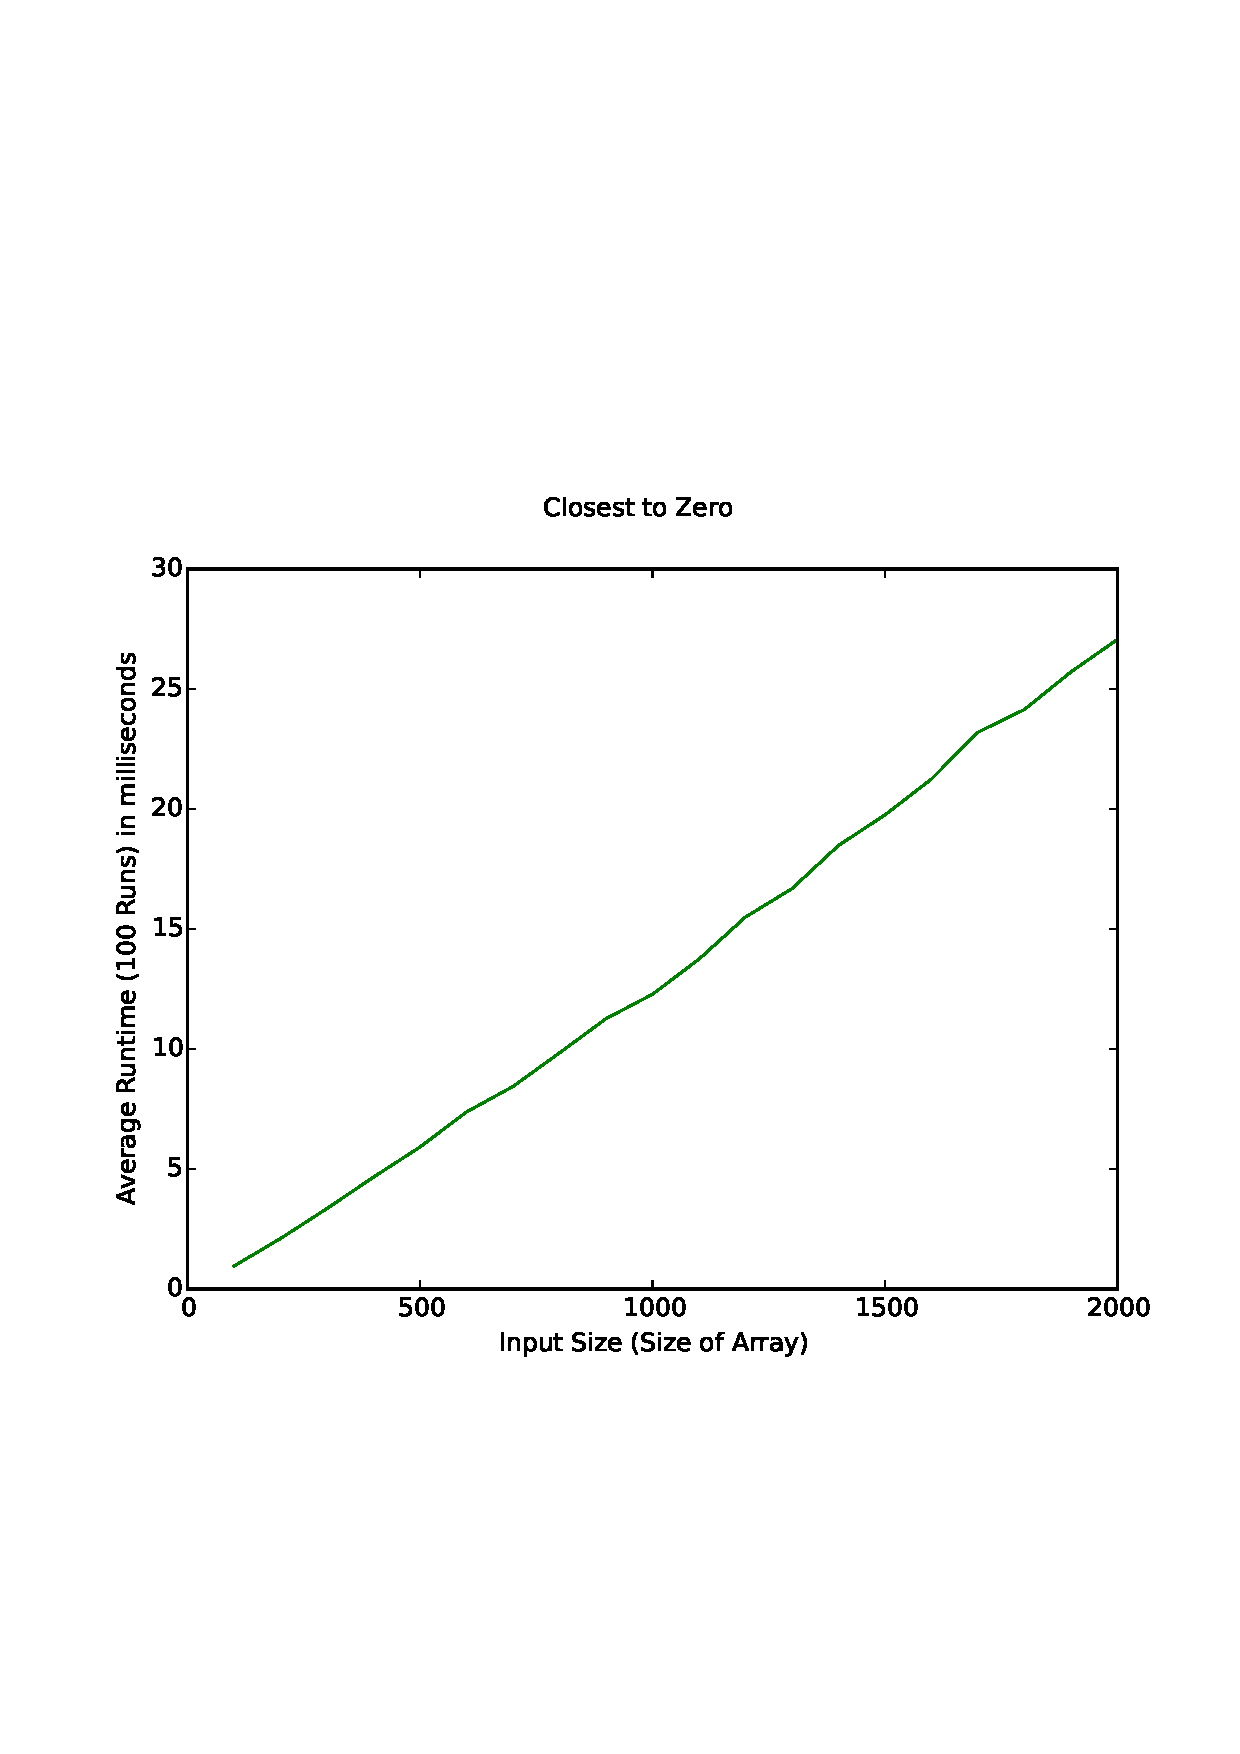
\includegraphics[width=\textwidth]{timings}


\end{document}
